\documentclass[11pt]{book}
\usepackage[colorlinks = true,linkcolor = blue]{hyperref}
\usepackage[letterpaper]{geometry} % Custom margins
\usepackage{graphicx}
\usepackage{tabularx}
\usepackage{float}
\usepackage[spanish]{babel}
\usepackage[T1]{fontenc}
\usepackage[utf8]{inputenc}
\usepackage{remreset}
\usepackage{enumitem}
\usepackage{xparse}
\usepackage{wrapfig}
\usepackage{amssymb,amsmath}
\usepackage{tikz}
\usetikzlibrary{
  arrows,
  positioning,
  matrix,
  calc,
  decorations.pathreplacing,
  decorations.pathmorphing,
  decorations.markings,
  decorations.text,
  shapes,
  backgrounds,
  shadows,
  trees,
  fit,
  snakes,
  patterns,
  mindmap,
  intersections,
  calendar,
  plotmarks,
  spy,
  tikzmark}
  
  \decimalpoint

%%%% APRENDISAJES TEXTBOX
\tikzset{
  abstractbox/.style={
    draw=black, fill=white, rectangle, 
    inner sep=12pt, style=rounded corners,
    drop shadow={fill=black, opacity=1}
  },
  abstracttitle/.style={fill=white}
}
\newcommand{\boxabstract}[2][fill=white]{
  \begin{tikzpicture}
    \node [abstractbox, #1] (box)
    {\begin{minipage}{0.9\linewidth}
        \setlength{\parindent}{2mm} % Indentar.
        \normalfont #2
      \end{minipage}};
    \node[abstracttitle, right=10pt] at (box.north west) {Aprendizajes esperados:};
    \node[draw=none, fit=(box)] {};
  \end{tikzpicture}
}
%%%%%%%%%%%%%%%%%%%%%%%%

\makeatletter
  \@removefromreset{section}{chapter}
\makeatother
\addto\captionsspanish{\renewcommand{\chaptername}{}}
\renewcommand{\thechapter}{Unidad \arabic{chapter}}
\renewcommand{\thesection}{S\arabic{section}}
\renewcommand{\thesubsection}{L\arabic{subsection}}
\setlength{\parindent}{0pt}

\begin{document}
\pagestyle{empty}
\newgeometry{letterpaper,left=15mm,top=50mm,bottom=0mm} % Custom margins
\begin{center}
  {\Huge Matem\'aticas 1}\\
  \vspace{2cm}
  \normalsize
  \textbf{\large Cuaderno de trabajo}\\
  para los alumnos de 1$^\circ$ de  Secundaria\\
  en el curso durante el ciclo escolar\\
  \textbf{2022-2023}\\
  \vspace{2.5cm}
  \small POR\\
  \Large J. C. Melchor Pinto\\[0.5em]
  \normalsize Profesor de asignatura en\\
  \vspace{1cm}
  
\includegraphics[width=4cm]{./Unidad 2/Images/LOGO_RDS_nobg}
\end{center}
\vspace{2cm}
%\include*{Functional/TitlePage}
\hspace{-16mm}
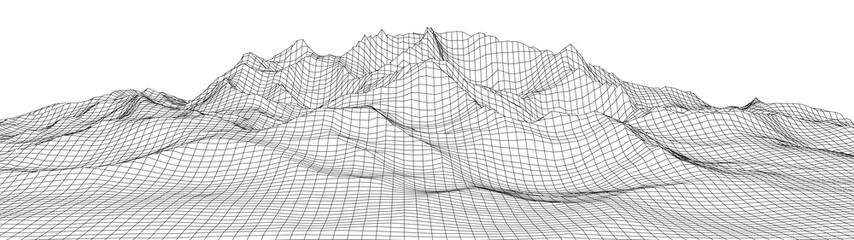
\includegraphics[width=\paperwidth]{./Unidad 2/Images/cover_bg_short}
\restoregeometry
\tableofcontents
\chapter{}
\section{Fracciones y decimales}
\subsection{Equivalencias de fracciones y decimales}
\subsection{Decimales peri\'odicos}
\subsubsection{Redondeo y truncamiento}

\section{Recta Num\'erica, Densidad y Orden}
\subsection{Fracciones en la Recta Num\'erica, Densidad y Orden}
\subsection{Decimales en la Recta Num\'erica, Densidad y Orden}
\subsection{Orden de fracciones y decimales}
\subsubsection{Orden en los n\'umeros fraccionarios}
\subsubsection{Orden en los n\'umeros decimales}

\section{Problemas con sumas y restas}
\subsection{N\'umeros con signo, recta y orden}
\subsection{Suma y resta de n\'umeros con signo}
\subsubsection{Suma de numeros con signo}
\subsubsection{Conmutatividad aditiva}
\subsubsection{Resta de n\'umeros con signo}

\section{Multiplicaci\'on con n\'umeros fraccionarios y decimales}
\subsection{Multiplicaci\'on con n\'umeros fraccionarios}
\subsection{Multiplicaci\'on con n\'umeros decimales}

\section{Divisi\'on con n\'umeros fraccionarios y decimales}

\section{\'Angulos, tri\'angulos y cuadril\'ateros}
\subsection{\'Angulos y rectas paralelas}
\subsection{Suma de los \'angulos interiores de un tri\'angulo y de un cuadril\'atero}
\subsubsection{\'Angulos de un tri\'angulo}
\subsubsection{\'Angulos de un cuadril\'atero}

\section{Tri\'angulos, cuadril\'ateros y congruencia}
\subsection{Criterios de congruencia}





\chapter{}

\section{Jerarqu\'ia de operaciones y signos de agrupaci\'on}
\boxabstract{
  Lee con atenci\'on cada pregunta y realiza lo que se te pide.
  De ser necesario, desarrolla tus respuestas en el espacio
  determinado para cada pregunta o
  en una hoja en blanco por separado, anotando en ella tu nombre
  completo, el n\'umero del problema y la soluci\'on propuesta.
}
\subsection{Jerarqu\'ia de operaciones y signos de agrupaci\'on}
Dentro de las operaciones básicas de la aritmética existe una \textbf{jerarquía de operaciones}, es decir un \textbf{orden}.

Recuerda cuando estabas en primaria y empezabas a leer, ¿qué aprendiste primero?. Seguro fueron las vocales, después fueron sílabas, después palabras completas hasta poder llegar a los enunciados y dentro de los enunciados vienen los signos de puntuación, las comas, los dos puntos, el punto y seguido, el punto aparte, etc. Y entendiste la importancia de los signos de puntuación.

En el siguiente enunciados podemos observar ejemplos:

Perdón imposible, castigarlo.\\
Perdón, imposible castigarlo.

Como podemos ver el significado de ambas expresiones son diferentes, bueno de eso se trata, en las matemáticas existen reglas que si no se siguen el resultado de la operación sería incorrecto.

La operación de suma, resta, multiplicación y división tienen el siguiente orden:
\begin{figure}[H]
  \centering
  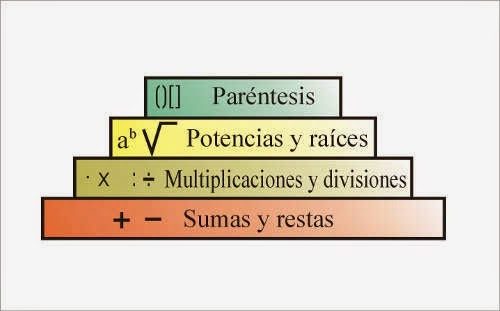
\includegraphics[width=0.5\textwidth]{./Unidad 2/Images/jerarquia.jpg}
\end{figure}

\subsubsection{Ejemplo 1: En este ejercicio aremos el uso del paréntesis}

\[( 10 + 2 ) / 3 - 2\]

Observemos en este primer ejemplo se tiene un paréntesis y tiene mayor jerarquía, por lo que primero se realiza esta operación.

\[12 / 3 - 2\]

Seguimos con el operador que tiene la jerarquía mas alta que es la división, y vamos de izquierda a derecha y realizamos la operación.

\[4 - 2\]

Y por último, al resultado se le restan 2. Por lo que la operación nos queda:

\[( 10 + 2 ) / 3 - 2 = 2\]



\subsubsection{Ejemplo 2: En este ejercicio no utilizaremos el paréntesis}


Ahora vamos a ver el mismo problema pero sin el paréntesis.

\[5 + 6 / 2 - 2\]

Observemos que ahora la jerarquía mas alta la tiene primero la división, ya que no existe ningún paréntesis.

\[8 + 2 - 2 = 8\]

Vamos de izquierda a derecha, hacemos primero la suma y luego la resta y tenemos el resultado, como podemos apreciar la gran importancia de respetar el orden de las operaciones para poder encontrar el resultado correcto.


\subsubsection{Ejemplo 3: En este ejercicio explicaremos un poco más detallado}

\[4 - 6 / 2 + 5 \times 2\]

Vamos de izquierda a derecha y hacemos la división por que en este ejemplo es el operador con mas jerarquía.

\[4 - 3 + 5 \times 2\]

Luego vamos de izquierda a derecha buscando el operador que tiene la mayor jerarquía para hacer la operacion. el cual es la multiplicaciónn.

\[4 - 3 + 10\]

Seguimos con la resta por izquierda y luego por la derecha

\[1 + 10\]

Por ultimo el resultado es el número 11.

\[4 - 6 / 2 + 5 \times 2 = 11\]

\section{Resolución de problemas con valores faltantes}

\subsection{Proporcionalidad directa y valor faltante}
\subsection{Proporcionalidad y valor unitario}
\subsection{Resolución de problemas de proporcionalidad directa}


\section{Porcentajes}
\subsection{Tanto por ciento}
\subsection{Cálculo del porcentaje}
\subsection{Porcentajes y aplicaciones}

\section{Perímetros y áreas}
\subsection{Perímetro de polígonos}
\subsection{Perímetro del círculo}
\subsection{Áreas de triángulos y cuadriláteros}

\section{Ecuaciones lineales}
\subsection{Formulación de ecuaciones}
\subsection{Solución de una ecuación}

\section{Resolución de ecuaciones lineales}
\subsection{Propiedades de la igualdad}
\subsection{Más sobre ecuaciones lineales}

\section{Medidas de tendencia central}
\subsection{Media aritmética o promedio}
\subsection{La media aritmética y el rango}

\section{Moda, media aritmética y mediana}
\subsection{Media aritmética y mediana}
\subsection{Moda}
\subsection{Representantes de un grupo de datos}

\chapter{}

\section{Situaciones de variación proporcional}
\subsection{Comparación de situaciones de variación proporcional con tablas}
\subsection{Comparación de situaciones de variación proporcional con gráficas}
\subsection{Comparación de situaciones de variación proporcional con expresiones algebraicas}

\section{Pendiente de una recta y razón de cambio}
\subsection{Variación proporcional y pendiente}
\subsection{Razón de cambio y variación}
\subsection{Efectos en la recta al cambiar la pendiente}

\section{Análisis y comparación de situaciones de variación lineal}
\subsection{Efectos de la recta al cambiar la ordenada al origen}
\subsection{Situaciones de variación lineal asociadas a la física, la biología y la economía}

\section{Sucesiones y expresiones algebraicas}
\subsection{Sucesiones numéricas}
\subsection{Sucesiones con progresión aritmética}

\section{Congruencia de triángulos y aplicaciones}
\subsection{Aplicaciones de congruencia de triángulos}
\subsection{Aplicaciones a cuadriláteros}

\section{Vol\'umenes de prismas rectos}
\subsection{Volumen de prismas rectos rectangulares}
\subsection{Fórmula del volumen de prismas rectos}

\section{Gráficas circulares}
\subsection{Recolecta y registra datos}
\subsection{Registra datos en gráficas circulares}
\subsection{Leer e interpretar datos en gráficas circulares}

\section{El azar y la probabilidad frecuencial}
\subsection{Tipos, recolección y organización de datos}
\subsection{Experimentos aleatorios y deterministas}
\subsection{Espacio muestral de un experimento aleatorio}
\subsection{Cálculo de la probabilidad frecuencial}






\end{document}





